\documentclass{article}

\title{AI5006 - Assignment 1}
\author{Addagalla Satyanarayana - AIRESCH14003 }
\date{September-06-2020}
\usepackage{geometry}
\geometry{
	a4paper,
	total={170mm,257mm},
	left=20mm,
	top=5mm,
}
\usepackage{graphicx}
\usepackage{amsmath}
\usepackage{mathtools}
\usepackage{nccmath}
\begin{document}
	\maketitle
	\section*{Question :}

{\Large Find the vector equation of the line passing through the point 	
$\begin{psmallmatrix}1 \\2 \\-4	\end{psmallmatrix}$
and perpendicular to the two lines

$\frac{x-8}{3} = \frac{y+19}{-16}= \frac{z-10}{7} $ and\\\\
$\frac{x-15}{3} = \frac{y-29}{8}= \frac{z-5}{5} $\\

\section*{Solution :}

Equation of a $\vec{\textbf{l}}$ passing through $\vec{\textbf{a}}$ and parallel to  $\vec{\textbf{n}}$ is given by:\\\\
$\vec{\textbf{l}} =\vec{\textbf{a}} + L*\vec{\textbf{n}} $, where L is some constant

Since the line passes through $\begin{psmallmatrix}	1 \\2 \\-4\end{psmallmatrix} \\
\vec{\textbf{a}} = (i + 2j - 4k)$

Let $\vec{\textbf{n}}$ be the normal vector to both lines. If $\vec{\textbf{m}_\textbf{1}}$ and $\vec{\textbf{m}_\textbf{2}}$ are the direction vectors of the lines,then

$\vec{\textbf{m}_\textbf{1}}^T\vec{\textbf{n}} = 0$

$\vec{\textbf{m}_\textbf{2}}^T\vec{\textbf{n}} = 0$

Let $\vec{\textbf{n}} = \begin{pmatrix} x \\ y \\ z\end{pmatrix} $
$\vec{\textbf{m}_\textbf{1}} = \begin{pmatrix} 3 \\ -16 \\ 7\end{pmatrix} $
$\vec{\textbf{m}_\textbf{2}} = \begin{pmatrix} 3 \\ 8 \\ -5\end{pmatrix} $\\\\
Since  $\vec{\textbf{n}}$ is perpendicular to $\vec{\textbf{m}_\textbf{1}}$ and $\vec{\textbf{m}_\textbf{2}}$ \\
$3x -16y + 7z = 0$\\ 
$3x + 8y - 5z = 0$\\

Solving the equations
$\frac{x}{2} = \frac{y}{3}= \frac{z}{6} = K$\\
$ x = 2K , y = 3K , z =6K$

$\vec{\textbf{n}} =K* (2i + 3j + 6k)$

so the equation of  $\vec{\textbf{l}}$ is\\
$\vec{\textbf{l}}=(i + 2j - 4k) + L*K (2i + 3j + 6k)$ ,where L*K is any constant\\

\begin{figure*}[hb]
	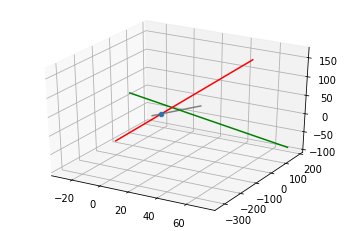
\includegraphics[width=\linewidth]{assignment1.png}
	\caption{perpendicular}
	\label{fig:1}
\end{figure*}
\end{document}